\documentclass[10pt,twocolumn]{article}

\usepackage[utf8]{inputenc}
\usepackage[T1]{fontenc}
\usepackage{lmodern}
\usepackage{microtype}
\usepackage[margin=0.72in,top=0.78in,bottom=0.78in,columnsep=0.26in]{geometry}
\usepackage{amsmath,amssymb}
\usepackage{booktabs}
\usepackage{graphicx}
\usepackage{xcolor}
\usepackage{hyperref}
\usepackage[numbers,sort&compress]{natbib}
\usepackage{caption}
\usepackage{titlesec}
\usepackage{enumitem}
\setlist{nosep,leftmargin=*}

\definecolor{navy}{HTML}{1B365D}
\hypersetup{
  colorlinks=true,
  linkcolor=navy,
  citecolor=navy,
  urlcolor=navy,
  pdftitle={Illusions of Impunity: Deconfounding Fixture Quality, Non-Foul Intercepts, Spatial Placement, and Small-Sample Noise in Association Football Disciplinary Ratios},
  pdfauthor={Pedro Vidigal}
}

\captionsetup{font=small,labelfont=bf}
\titlespacing*{\section}{0pt}{1.6ex plus 0.4ex minus 0.2ex}{0.8ex plus 0.2ex}
\titlespacing*{\subsection}{0pt}{1.2ex plus 0.3ex minus 0.1ex}{0.5ex plus 0.1ex}

\title{\vspace{-1.2em}\textbf{Illusions of Impunity: Deconfounding Fixture Quality, Non-Foul Intercepts, Spatial Placement, and Small-Sample Noise in Association Football Disciplinary Ratios}}

\author{
  \textbf{Pedro Vidigal}\\
  Independent Researcher, Lisbon, Portugal\\
  \texttt{pedro@pedrovidigal.com}
}

\date{October 2026 \quad$\cdot$\quad Target Venue: \textit{Journal of Quantitative Analysis in Sports (JQAS)} / \textit{MIT Sloan SSAC 2027}}

\begin{document}
\maketitle

\begin{abstract}
Public and media controversies in association football routinely cite a club's ratio of yellow cards to fouls committed as evidence of refereeing bias or tactical impunity. Across a four-study empirical programme combining $58,013$ completed-season matches across $11$ European top divisions ($2000\text{--}2025$), $2,737$ harvested Portuguese referee appointments, $47,955$ spatio-temporally coded fouls from five major leagues, and $3,100$ historical four-match season openings, we show that raw cards-per-foul ratios are systematically confounded at four distinct levels. First, an audit of $286$ league-season files demonstrates that $107$ files return valid tables with zero match statistics while referee identifiers are absent in $9$ of $11$ leagues, necessitating within-match conditioning and external official harvesting. Second, a club's raw booking index is confounded by pre-match win expectation ($31.3\%$ underdog-to-favourite swing in Portugal; $1.098$ vs.\ $0.856$ median across $11$ leagues) and by non-foul card intercepts ($13\%\text{--}47\%$ of yellow cards arise from dissent, time-wasting, and simulation, causing observed yellows-per-foul to fall monotonically from $0.197$ at $\le 6$ fouls to $0.122$ at $>20$ fouls). Crucially, computing the identical index for a club's \emph{opponents} reveals that team strength increases the opponent's booking index ($r = +0.283, p = 6.6\times 10^{-6}$) and that holding club identity fixed across opponent-strength terciles raises booking rates in $11$ of $11$ leagues ($0.938 \to 0.993 \to 1.088$): card intensity belongs to fixture quality rather than club favouritism. After leave-one-club-out referee and situation adjustment in Portugal, FC Porto ($0.890 \to 1.002$) and SL Benfica ($0.885 \to 1.002$) sit exactly at expectation, while only Sporting CP ($1.177$, Benjamini--Hochberg $p = 0.0004$) separates among $26$ clubs. Third, at the individual foul level ($N = 47,955$), card risk drops $3.5$-fold from a team's own defensive fifth ($31.4\%$) to the attacking fifth ($8.9\%$) and resets by $-3.3$ percentage points across half-time ($16.1\% \to 12.8\%, p = 4.1\times 10^{-4}$), yet $98$ Big-Five clubs compress into $[48.2, 58.0]$ in mean foul position ($r = -0.143$, inside a $2,000$-draw matched spatial-Poisson null of $\bar{r} = -0.210, [-0.397, -0.015]$). Even restricting to late-game ($\ge 70'$), close-score ($0$ or $+1$) defensive/middle-third fouls ($4,547$ fouls, $25.7\%$ carded) explains only $0.3\%$ of between-club variance ($r = +0.053$). Fourth, across $2,528$ consecutive club-season pairs, only $15.1\%$ of single-season variance is true club signal ($r = +0.324$ vs.\ Poisson null maximum $+0.056$), so ignoring a club's one-season ratio in favour of the league mean lowers next-season prediction error by $11.6\%$ (and Empirical-Bayes shrinkage by $13.3\%$), while all $31$ historical bottom-$1\%$ four-match openings reverted to a rest-of-season median of $0.965$.
\end{abstract}

\section{Introduction}

In professional association football, disciplinary statistics---fouls committed and yellow or red cards issued---are the most widely available behavioural records outside goals and shots. Because raw counts of fouls and bookings are published for almost every modern top-flight match, analysts, club officials, and supporters frequently construct a simple ratio: yellow cards per foul committed (or its reciprocal, fouls per card). When a dominant domestic club accumulates a low ratio of cards to fouls, the discrepancy is routinely interpreted either as institutional favouritism by match officials or as a deliberate tactical skill: committing fouls in pitch zones or match states where referees are reluctant to book \citep{phatak2021dirty,azmat2024xb}.

This paper demonstrates that reasoning directly from an aggregate cards-to-fouls ratio to a club-level behavioural or officiating claim commits a sequence of four methodological errors:
\begin{enumerate}
  \item \textbf{Silent schema and denominator traps (Study 01):} Public football repositories exhibit severe longitudinal truncation, unrecorded rule differences in second-yellow accounting, and missing referee identifiers across $9$ of $11$ European leagues.
  \item \textbf{Proportional misspecification and fixture-level confounding (Study 02):} Yellow cards are an affine rather than proportional function of fouls because conduct offences (dissent, delaying restarts, simulation) enter as a positive intercept ($13\%\text{--}47\%$ of cards). Moreover, conditioning on pre-match strength and testing the \emph{opponents'} booking index proves that elevated card-per-foul rates are a property of high-quality fixtures for \emph{both} teams on the pitch.
  \item \textbf{Event-to-actor ecological compression (Study 03):} Although the spatial and temporal card gradient at the level of an individual foul is steep ($31.4\%$ in the defensive fifth vs.\ $8.9\%$ in the attacking fifth; $25.7\%$ in late-game close-score defensive/middle-third situations vs.\ $14.2\%$ outside), clubs stand in nearly the same place on the pitch ($[48.2, 58.0]$ mean $x$-coordinate), leaving $91.2\%$ of between-club variation unexplained even on the most favourable tail statistic.
  \item \textbf{Small-sample Poisson dominance (Study 04 \& Sealed Protocol):} Across $2,528$ consecutive club-season pairs, $84.9\%$ of the cross-sectional variance in a single season's adjusted booking index is Poisson sampling noise. Consequently, a club's own one-season raw ratio is outperformed as an out-of-sample predictor of its next season by $11.6\%$ simply by predicting the league mean, and by $13.3\%$ via Empirical-Bayes shrinkage \citep{efron1975stein,brown2008season}.
\end{enumerate}

Every empirical claim in this paper is bound by continuous-integration tests to deterministic JSON sidecars and Parquet snapshots committed in an open repository, accompanied by a six-attack adversarial pressure-test matrix (specification, aggregation, adjustment coarseness, prior work, baseline sufficiency, and cross-sectional unit count) and a sealed out-of-sample pre-registration tracking an extreme $2026\text{--}27$ four-match opening ($58$ fouls, $1$ yellow card).

\section{Related Work}

\textbf{Referee bias, social pressure, and team strength.} A rich econometric and sports-science literature examines officiating in football. \citet{garicano2005favoritism} and \citet{dohmen2008social} established that referees adjust injury time in response to score state and crowd pressure, while \citet{boyko2007referee} and \citet{sors2021silence} documented home-crowd effects on disciplinary sanctions that attenuated in spectator-free matches. Most relevant to our Study~02, \citet{dawson2007referees} analysed $2,660$ English Premier League matches ($1996\text{--}2003$) using a bivariate Negative Binomial and Nash-equilibrium aggression model, finding significant referee-to-referee inconsistency alongside a team-strength gradient in total bookings. We extend \citet{dawson2007referees} to $58,013$ matches across $11$ leagues while conditioning explicitly on foul volume and decomposing own versus opponent indices within the same fixture.

\textbf{Fouling incentives, spatial risk, and Simpson's paradox.} \citet{wright2003professional} modelled when a professional foul is tactically rational, and \citet{ridder1994down} estimated the scoring cost of red-card dismissals. \citet{phatak2021dirty} compared fouls-per-card across five European leagues and demonstrated Simpson's paradox \citep{simpson1951interpretation} when pooling across leagues with distinct officiating baselines. At the individual event level, \citet{pappalardo2019events} released spatio-temporal event logs for the $2017\text{--}18$ Big-Five European seasons, and \citet{azmat2024xb} formulated an Expected Booking ($\text{xB}$) model of $P(\text{card}\mid\text{foul context})$. While \citet{azmat2024xb} establish that event context predicts whether \emph{a} foul is carded, our Study~03 tests whether real clubs actually separate along that gradient.

\textbf{Reliability, shrinkage, and false discovery.} Separating persistent skill from random noise in sports metrics relies on split-half reliability \citep{cronbach1951alpha}, Empirical-Bayes shrinkage \citep{efron1975stein,brown2008season}, partial pooling \citep{gelman2012multiple}, and False Discovery Rate (FDR) control \citep{benjamini1995controlling}, alongside guards against regression-to-the-mean artifacts \citep{barnett2005regression} and undisclosed researcher degrees of freedom \citep{simmons2011false,ioannidis2005why,peng2011reproducible}. \citet{johnson2010stable} raised the profile-stabilisation question for football match indicators; our Study~04 provides the exact variance decomposition and out-of-sample shrinkage validation for disciplinary indices across $11$ leagues.

\section{Study 01: Provenance and Structural Limits of Public Match Data}

Before fitting any disciplinary model, we audited the primary open archive of match-level European football statistics (\texttt{football-data.co.uk}) across $11$ top divisions---England (\texttt{E0}), Scotland (\texttt{SC0}), Germany (\texttt{D1}), Italy (\texttt{I1}), Spain (\texttt{SP1}), France (\texttt{F1}), Netherlands (\texttt{N1}), Belgium (\texttt{B1}), Portugal (\texttt{P1}), Turkey (\texttt{T1}), and Greece (\texttt{G1})---over $26$ completed seasons ($2000\text{--}01$ through $2025\text{--}26$), comprising $286$ league-season CSV files \citep{wilkinson2016fair,gebru2021datasheets}.

\begin{table}[t]
\centering
\caption{Audit of $286$ completed league-season files across $11$ European top divisions ($2000\text{--}01$ to $2025\text{--}26$, snapshot \texttt{2026-W35}; $N = 58,013$ matches with fouls and cards).}
\label{tab:study01}
\footnotesize
\setlength{\tabcolsep}{4.2pt}
\resizebox{\columnwidth}{!}{%
\begin{tabular}{@{}lccc@{}}
\toprule
\textbf{League} & \textbf{Fouls \& Cards} & \textbf{Usable Files} & \textbf{Referee Column} \\
\midrule
England (\texttt{E0}) & $2000\text{--}2025$ & $26 / 26$ & $2000\text{--}2025$ ($26$) \\
Scotland (\texttt{SC0}) & $2000\text{--}2025$ & $26 / 26$ & $25 / 26$ (no $12\text{--}13$) \\
Germany (\texttt{D1}) & $00\text{--}01, 03\text{--}25$ & $25 / 26$ & $2000\text{--}2001$ only ($2$) \\
Italy (\texttt{I1}) & $2005\text{--}2025$ & $21 / 26$ & $2005\text{--}2006$ only ($2$) \\
Spain (\texttt{SP1}) & $2005\text{--}2025$ & $21 / 26$ & Never ($0$) \\
France (\texttt{F1}) & $2007\text{--}2025$ & $19 / 26$ & Never ($0$) \\
Netherlands (\texttt{N1}) & $2017\text{--}2025$ & $9 / 26$ & Never ($0$) \\
Portugal (\texttt{P1}) & $2017\text{--}2025$ & $9 / 26$ & Never ($0$) \\
Turkey (\texttt{T1}) & $2017\text{--}2025$ & $9 / 26$ & Never ($0$) \\
Belgium (\texttt{B1}) & $2019\text{--}2025$ & $7 / 26$ & Never ($0$) \\
Greece (\texttt{G1}) & $2019\text{--}2025$ & $7 / 26$ & Never ($0$) \\
\midrule
\textbf{Total} & \textbf{58,013 matches} & \textbf{179 / 286} & \textbf{55 / 286 files} \\
\bottomrule
\end{tabular}%
}
\end{table}

Table~\ref{tab:study01} summarises four structural findings that constrain any valid multi-league disciplinary study:
\begin{enumerate}
  \item \textbf{Silent absence of match statistics:} Only $179$ of $286$ league-season files ($62.6\%$) contain foul and card columns ($58,013$ completed matches; $190$ files when including the in-progress $2026\text{--}27$ snapshot). The remaining $107$ files download with HTTP~$200$ and parse cleanly into DataFrames containing only scores and betting odds. In Portugal, Netherlands, and Turkey, foul and card records begin only in $2017\text{--}18$ ($9$ completed seasons); in Belgium and Greece, in $2019\text{--}20$ ($7$ seasons).
  \item \textbf{Interrupted series:} Germany carries fouls, cards, and referee identities in $2000\text{--}01$ and $2001\text{--}02$, drops all match statistics in $2002\text{--}03$, and resumes fouls and cards (without referees) from $2003\text{--}04$.
  \item \textbf{Referee coverage contraction:} Match-official identity is recorded continuously only in England and Scotland (bar $2012\text{--}13$), for two seasons each in Germany and Italy, and never in the other seven leagues.
  \item \textbf{Schema widening without event expansion:} While the median file width more than quintupled from $25$ columns in $2000\text{--}01$ to $131$ columns in $2025\text{--}26$ due to bookmaker odds proliferation, columns describing pitch events rose from $0$ to $12$ by $2007$ and have remained frozen for nineteen years. Moreover, two definitional traps prohibit cross-league pooling: English and Scottish feeds exclude the first yellow card of a second-bookable dismissal whereas continental feeds count both, and match-level yellow-card totals include non-foul bookings (dissent, time-wasting, bench sanctions).
\end{enumerate}

\section{Study 02: Deconfounding the Club Booking Index}

\begin{figure*}[t]
\centering
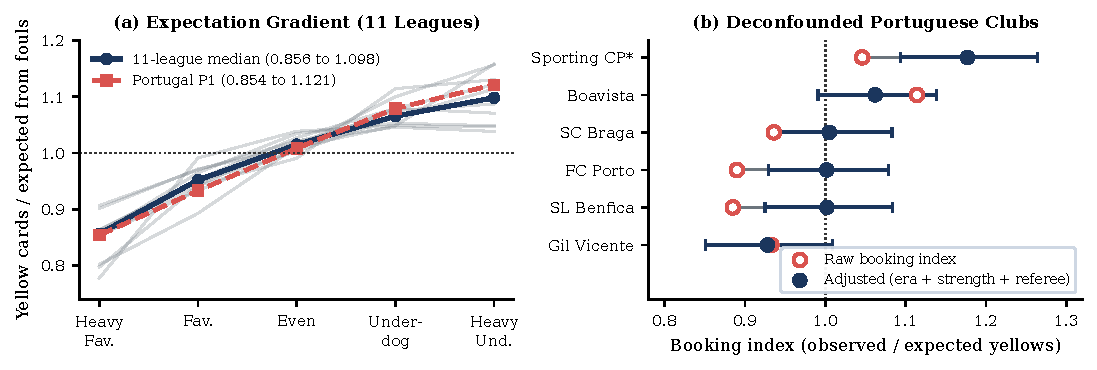
\includegraphics[width=\textwidth]{figures/fig1.pdf}
\caption{\textbf{Study 02: Match-expectation gradient and club-level deconfounding.} \textbf{(a)} Ratio of observed yellow cards to fouls-implied expectation across five pre-match win-probability bands in $11$ European leagues ($N = 58,013$ matches); heavy underdogs are booked at $1.098\times$ median expectation vs.\ $0.856\times$ for heavy favourites ($1.121$ vs.\ $0.854$ in Portugal, a $31.3\%$ swing). \textbf{(b)} Raw vs.\ era-, situation-, and leave-one-club-out referee-adjusted booking indices across Portuguese clubs ($N = 2,737$ official appointments, $95\%$ CIs). FC Porto ($0.890 \to 1.002$) and SL Benfica ($0.885 \to 1.002$) collapse to the league average; only Sporting CP ($1.177$, BH $p = 0.0004$) separates.}
\label{fig:fig1}
\end{figure*}

Motivated by a viral public claim that FC Porto were systematically favoured by Portuguese referees based on a low raw cards-per-foul ratio, we pre-registered a test of whether any club in the Portuguese Primeira Liga (\texttt{P1}) exhibits an anomalous booking rate relative to the fouls it commits, and subjected the estimator to six adversarial pressure tests across all $11$ European leagues ($58,013$ matches, $115,946$ team-match observations).

\subsection{The Naive Estimator and Its Four Failures}
Let $Y_{i,m}$ and $F_{i,m}$ denote the yellow cards received and fouls committed by team $i$ in match $m$. Under a naive proportional model $E_0[Y_{i,m}] = \bar{r}_{L,s} F_{i,m}$ (where $\bar{r}_{L,s} = \sum Y / \sum F$ within league $L$ and season $s$), FC Porto's ten-season raw booking index $I^{\text{raw}}_i = \sum Y_{i,m} / \sum E_0[Y_{i,m}]$ is $0.890$ and SL Benfica's is $0.885$---both roughly $11\%$ below parity ($1.000$). Four sequential diagnostics show why this raw index is an artifact.

\textbf{Failure 1: Pre-match strength and match expectation.} Using pre-match bookmaker odds (and Elo ratings where odds are absent) to compute each side's pre-match strength differential $s_{i,m}$, Figure~\ref{fig:fig1}(a) partitions all $115,946$ team-match rows into five expectation bands. In Portugal, a heavy underdog is booked at $1.121\times$ its foul-implied expectation whereas a heavy favourite is booked at $0.854\times$---a $31.3\%$ swing with no club identity in the model. Across all $11$ European leagues, the heavy-underdog band exceeds the heavy-favourite band in $11$ of $11$ competitions (median $1.098$ vs.\ $0.856$, strictly monotone across all five bands in $7$ of $11$ leagues). Because domestic giants are favourites in most fixtures, attributing the favourite discount to club-specific referee bias confounds club identity with match situation.

\begin{figure*}[t]
\centering
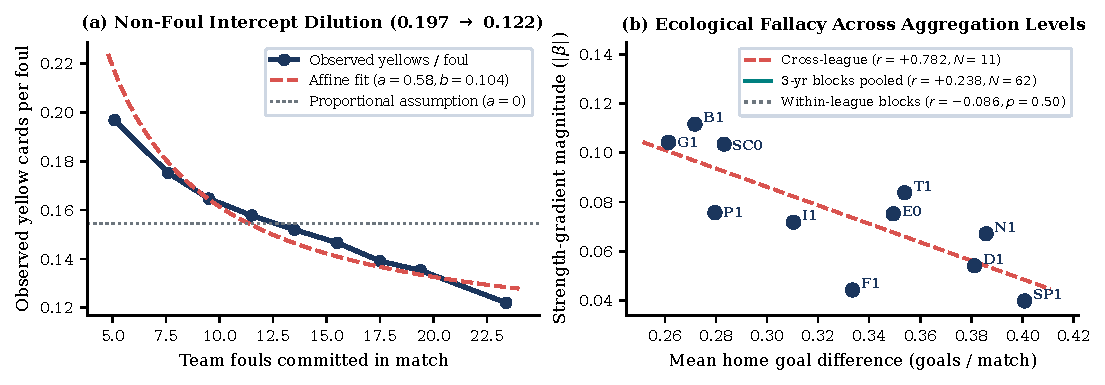
\includegraphics[width=\textwidth]{figures/fig2.pdf}
\caption{\textbf{Study 02: Non-foul intercept dilution and multi-level ecological reversal.} \textbf{(a)} Observed yellow cards per foul across team foul-count bins ($N = 115,946$ team-matches), declining monotonically from $0.197$ at $\le 6$ fouls to $0.122$ at $>20$ fouls because non-foul conduct cards enter as a positive affine intercept $a > 0$ ($13\%\text{--}47\%$ of mean cards). \textbf{(b)} Cross-league correlation between strength-gradient magnitude and home goal difference ($r = +0.782, N = 11$) vanishes across pooled three-season blocks ($r = +0.238, N = 62$) and reverses sign within leagues over time ($r = -0.086, p = 0.504$, negative in $5$ of $6$ leagues).}
\label{fig:fig2}
\end{figure*}

\textbf{Failure 2: Affine misspecification and non-foul intercepts.} The proportional model assumes zero cards at zero fouls ($a = 0$). Fitting the affine specification $E[Y_{i,m}\mid F_{i,m}] = a_{L,s} + b_{L,s} F_{i,m}$ within each league-season reveals a positive intercept $a_{L,s}$ accounting for $13\%$ to $47\%$ of mean yellow cards across the $11$ leagues (reaching nearly half of all bookings in Greece and Italy). Figure~\ref{fig:fig2}(a) shows the empirical consequence: observed yellows per foul $Y/F = a/F + b$ declines monotonically with foul volume across all nine bins, from $0.197$ when a side commits $\le 6$ fouls ($5.1$ bin mean) to $0.122$ when it commits $>20$ fouls ($23.4$ bin mean). Cross-checking against the Wyscout event-coded sub-types in our Study~03 dataset (\texttt{typology.json}) confirms the physical mechanism: four non-challenge conduct labels (\emph{Protest}, \emph{Time lost foul}, \emph{Simulation}, and \emph{Out of game foul}) produce $642$ of the $7,346$ total cards ($8.74\%$ of all cards, carded at $99.1\%$), with individual club non-play card shares ranging from $1.5\%$ to $17.9\%$ (median $8.1\%$, split-half reliability $r = 0.251$, Spearman--Brown corrected $0.402$). Forcing the expectation line through the origin mechanically inflates low-foul dominant teams and deflates high-foul teams.

\textbf{Failure 3: The opponent test (fixture quality vs.\ club trait).} Once the affine expectation is adjusted continuously for pre-match strength, a club's long-run strength still correlates positively with its own adjusted booking index across the $246$ clubs in the $11$ leagues ($r = +0.484, p = 7.8\times 10^{-16}$; Spearman $\rho = +0.349$). However, computing the exact same adjusted booking index for each club's \emph{opponents} in the matches they play against that club yields $r = +0.283$ ($p = 6.6\times 10^{-6}$), while a club's own index and its opponents' index are nearly independent ($r = +0.116, p = 0.069$). Even more decisively, holding club identity fixed and partitioning each club's own matches into terciles of opponent quality shows that a team's booking index rises with the strength of the opponent it faces in $11$ of $11$ leagues: across the $11$-league median, a club is booked at $0.938$ against weakest-tercile opponents, $0.993$ against middle-tercile opponents, and $1.088$ against strongest-tercile opponents ($0.939 \to 0.973 \to 1.092$ in Portugal). Thus, yellows per foul scale with the quality of the \emph{fixture} for both teams. Testing whether the residual belongs to the head coach across $42$ multi-club managerial spell pairs in Portugal yields a null correlation of $r = -0.076$ ($5,000$-permutation $p = 0.628$).

\textbf{Failure 4: Ecological reversal across aggregation levels.} Across the $11$ league averages, the steepness of a league's strength gradient correlates with its mean home goal difference at $r = +0.782$ ($p = 0.0045$). Yet when the same panel is disaggregated into $62$ three-season blocks, Figure~\ref{fig:fig2}(b) shows the correlation dropping to $r = +0.238$ ($p = 0.063$) when pooled and reversing to $r = -0.086$ ($p = 0.504$, negative in $5$ of $6$ leagues with $\ge 4$ blocks) within leagues over time, despite home advantage falling from $0.349$ goals/match in $2001$ to $0.220$ in $2025$.

\subsection{Leave-One-Club-Out Referee Adjustment in Portugal}
Because \texttt{football-data.co.uk} omits Portuguese referees, we harvested $2,737$ official appointments across ten seasons and joined $98.4\%$ of them to our match records ($5,508$ team-matches) by date and scoreline validation. Among the $32$ Portuguese officials with $\ge 40$ matches, individual referee booking multipliers span $0.755$ to $1.324$---as wide as in England---but referee assignment across the $26$ ranked clubs ($\ge 80$ matches) is tightly balanced, with every club's mean referee draw lying between $0.971$ and $1.021$.

Estimating each referee's strictness multiplier $\hat{\rho}_{r,-i}$ \emph{excluding} all matches involving club $i$ (preventing a club's own card rate from contaminating its official baseline), Figure~\ref{fig:fig1}(b) and Table~\ref{tab:portugal_clubs} report the fully adjusted club booking indices:
\begin{itemize}
  \item \textbf{FC Porto:} Raw $0.890 \to$ situation-adjusted $1.018 \to$ referee-adjusted $\mathbf{1.002}$ ($95\%$ CI $[0.929, 1.079]$, two-sided $p = 0.964$, BH-adjusted $p = 0.965$).
  \item \textbf{SL Benfica:} Raw $0.885 \to$ situation-adjusted $1.009 \to$ referee-adjusted $\mathbf{1.002}$ ($95\%$ CI $[0.925, 1.084]$, raw $p = 0.965$, BH-adjusted $p = 0.965$).
  \item \textbf{Sporting CP:} Raw $1.046 \to$ situation-adjusted $1.179 \to$ referee-adjusted $\mathbf{1.177}$ ($95\%$ CI $[1.094, 1.264]$, raw $p = 1.6\times 10^{-5}$, BH-adjusted $p = 0.0004$, Bonferroni $p = 0.0004$).
\end{itemize}
Under Benjamini--Hochberg FDR control at $q = 0.10$ across all $26$ clubs, only Sporting CP separates; the runner-up (Gil Vicente, $0.928$, raw $p = 0.081$, BH $p = 0.635$) and third-ranked club (Boavista, $1.062$, raw $p = 0.090$, BH $p = 0.635$) are indistinguishable from sampling variation.

\begin{table}[t]
\centering
\caption{Deconfounded booking index for selected Portuguese clubs across ten seasons ($N = 5,508$ team-matches, $26$ clubs with $\ge 80$ matches, $2,737$ referee appointments).}
\label{tab:portugal_clubs}
\footnotesize
\setlength{\tabcolsep}{3.8pt}
\resizebox{\columnwidth}{!}{%
\begin{tabular}{@{}lcccccc@{}}
\toprule
\textbf{Club} & \textbf{Raw} & \textbf{Sit.\ Adj.} & \textbf{Ref.\ Adj.} & \textbf{95\% CI} & \textbf{Raw $p$} & \textbf{BH $p$} \\
\midrule
Sporting CP & $1.046$ & $1.179$ & $\mathbf{1.177}$ & $[1.094, 1.264]$ & $0.00002$ & $\mathbf{0.0004}$ \\
Boavista & $1.114$ & $1.067$ & $1.062$ & $[0.991, 1.138]$ & $0.090$ & $0.635$ \\
SC Braga & $0.936$ & $1.020$ & $1.005$ & $[0.931, 1.083]$ & $0.914$ & $0.965$ \\
FC Porto & $0.890$ & $1.018$ & $\mathbf{1.002}$ & $[0.929, 1.079]$ & $0.964$ & $0.965$ \\
SL Benfica & $0.885$ & $1.009$ & $\mathbf{1.002}$ & $[0.925, 1.084]$ & $0.965$ & $0.965$ \\
Gil Vicente & $0.933$ & $0.920$ & $0.928$ & $[0.851, 1.009]$ & $0.081$ & $0.635$ \\
\bottomrule
\end{tabular}%
}
\end{table}

\section{Study 03: The Spatial and Temporal Lever Nobody Pulls}

\begin{figure*}[t]
\centering
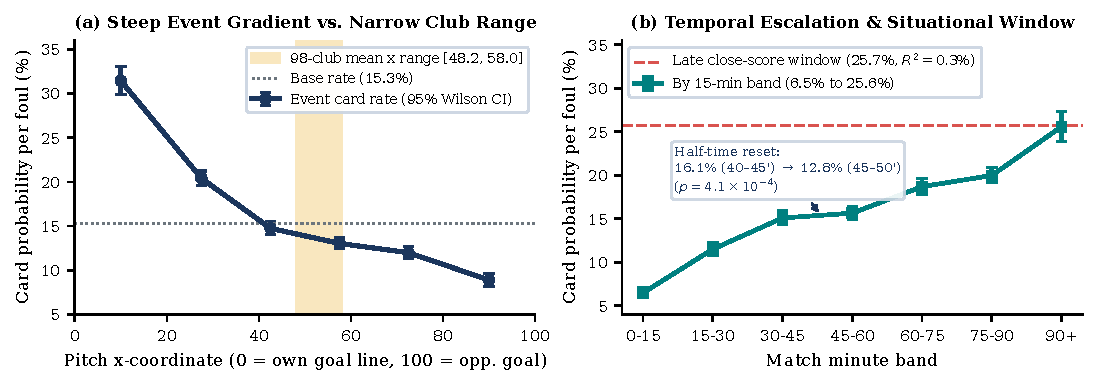
\includegraphics[width=\textwidth]{figures/fig3.pdf}
\caption{\textbf{Study 03: Event-level disciplinary gradients vs.\ club-level spatial compression ($N = 47,955$ fouls, $1,826$ matches, $98$ Big-Five clubs).} \textbf{(a)} Card probability per foul falls $3.5$-fold from a team's own defensive fifth ($31.4\%$) to the attacking fifth ($8.9\%$), but all $98$ clubs' season-mean foul $x$-coordinates compress into $[48.2, 58.0]$ (amber band), yielding $r = -0.143$ ($[-0.332, +0.057]$), indistinguishable from a $2,000$-draw matched spatial-Poisson null ($\bar{r} = -0.210, [-0.397, -0.015]$). \textbf{(b)} Temporal escalation from $6.5\%$ ($0\text{--}15'$) to $25.6\%$ ($90+'$), featuring a significant $-3.3\text{ pp}$ half-time reset ($16.1\% \to 12.8\%, p = 4.1\times 10^{-4}$) and a $25.7\%$ rate inside the late-game ($\ge 70'$), close-score ($0, +1$) defensive/middle-third tactical window ($R^2 = 0.3\%$ between clubs).}
\label{fig:fig3}
\end{figure*}

Could a club achieve a genuinely low card-per-foul rate by committing its fouls higher up the pitch or at safer moments? To test this mechanism at the event level, we analysed all $47,955$ fouls across $1,826$ matches and $98$ clubs ($\ge 200$ fouls each) in the $2017\text{--}18$ English, French, German, Italian, and Spanish top divisions from \citet{pappalardo2019events} (overall base card rate $15.32\%$).

\subsection{Steep Event Gradients and the Half-Time Discontinuity}
At the level of an individual foul, pitch location, elapsed time, and score state exert massive effects on card probability (Figure~\ref{fig:fig3}):
\begin{itemize}
  \item \textbf{Longitudinal and lateral location:} A foul in the fouling team's own defensive fifth ($x \le 20$) draws a card $\mathbf{31.4\%}$ of the time, compared with $\mathbf{8.9\%}$ in the attacking fifth ($x > 80$)---a $3.54\times$ ratio (ranging from $2.47\times$ in England to $4.97\times$ in Germany). By pitch thirds, card risk is $24.1\%$ in the defensive third, $14.0\%$ in the middle third, and $10.6\%$ in the attacking third ($22.8\%$, $12.7\%$, and $9.3\%$ when non-play conduct cards are removed). Central fouls ($|y - 50| \le 10$) are carded at $19.0\%$ versus $13.0\%$ wide ($|y - 50| > 40$).
  \item \textbf{Elapsed time and the half-time reset:} Card probability quadruples from $\mathbf{6.5\%}$ in the opening quarter-hour ($0\text{--}15'$) to $\mathbf{25.6\%}$ in second-half stoppage time ($>90'$). Crucially, the trajectory is not monotonic: card rate climbs to $\mathbf{16.1\%}$ in the final five minutes of the first half ($40\text{--}45'$), then drops by $\mathbf{3.3}$ percentage points to $\mathbf{12.8\%}$ in the opening five minutes of the second half ($45\text{--}50'$, $\chi^2$ contingency $p = 4.1\times 10^{-4}$). Because physiological fatigue does not discharge to first-half levels across a fifteen-minute interval, this discontinuity reflects within-half referee tolerance accumulation and reset.
  \item \textbf{Score state:} Fouls committed while trailing are carded at $\mathbf{18.1\%}$, while leading at $16.2\%$, and while level at $\mathbf{13.3\%}$.
\end{itemize}

\subsection{Why the Event Gradient Vanishes Between Clubs}
Despite a $3.5$-fold spatial gradient across the $100$-unit pitch, the season-average foul position across all $98$ Big-Five clubs spans only $\mathbf{48.2}$ to $\mathbf{58.0}$---less than one-tenth of the pitch (Figure~\ref{fig:fig3}(a)). Using \citet{cronbach1951alpha} split-variance reliability to net out within-club sampling error, $70.1\%$ of the between-club variance in mean foul $x$-position is genuine tactical variation (versus only $13.7\%$ for mean foul minute), and shifting from the worst to the best observed spatial-temporal foul mix among the $98$ clubs is worth $17.9\%$ of the base card rate ($16.6\%$ vs.\ $13.9\%$, and at most a $7.3\%$ reduction below a league's base rate in the most generous league, Spain).

Across the $98$ clubs, mean foul $x$-coordinate correlates with club card rate at $r = -0.143$ ($95\%$ CI $[-0.332, +0.057], p = 0.160$; $80\%$ power threshold $|r| = 0.28$), and an additive logistic regression in $(x, x^2, |y-50|, \text{minute}, \text{score state})$ explains only $\mathbf{3.1\%}$ of the between-club standard deviation in cards per foul.

\textbf{Matched spatial-Poisson and permutation nulls.} To separate ``no club exploits the spatial gradient'' from ``the observed $[48.2, 58.0]$ placement range is too narrow to overcome single-season Poisson noise,'' we executed two $2,000$-draw Monte Carlo nulls. Under a spatial-permutation null that randomly reassigns club mean $x$-positions across the $98$ clubs, $\bar{r} = +0.002$ ($95\%$ interval $[-0.193, +0.199]$, two-sided $p = 0.161$). Under a matched spatial-Poisson null where each club's actual foul coordinates in $[48.2, 58.0]$ are held fixed and club card totals are drawn from $\text{Poisson}(\sum_{j \in c} \hat{p}_{\text{spatial}}(x_j, y_j))$, the expected correlation is $\bar{r} = \mathbf{-0.210}$ with a $95\%$ sampling interval of $\mathbf{[-0.397, -0.015]}$. The observed $r = -0.143$ sits comfortably inside \emph{both} distributions: because clubs compress into a $9.8$-unit band near midfield, the mechanical slope induced by the spatial curve is smaller than the Poisson sampling noise of a $38$-match season.

\textbf{Tail-share versus volume proxy.} Replacing mean foul $x$ with a tail statistic---the share of a club's fouls committed in its own defensive third ($x < 33.3$, spanning $16.1\%$ to $29.9\%$ across the $98$ clubs)---strengthens the club-level correlation to $r = \mathbf{+0.296}$ ($95\%$ CI $[+0.103, +0.467]$, $R^2 = \mathbf{8.8\%}$; $r = +0.305, R^2 = 9.3\%$ on play-only fouls). Conversely, expressing defensive-third fouls as a per-match count ($1.76$ to $4.32$, median $3.07$) correlates with cards per match at $r = +0.670$ ($[+0.544, +0.766]$) solely because total fouls per match correlates with cards per match at $r = +0.696$ ($[+0.577, +0.786]$).

\textbf{Situational tactical-fouling interaction test.} A natural objection is that season averages mask cynical fouls committed in high-leverage moments: late in the match ($\text{minute} \ge 70$), in a close game ($\text{score\_diff} \in \{0, +1\}$), in the defensive or middle third ($x < 66.7$). Isolating this exact window captures $\mathbf{4,547}$ fouls ($9.5\%$ of all fouls), where the card rate jumps to $\mathbf{25.7\%}$ ($\mathbf{26.8\%}$ across the $2,069$ fouls committed while protecting a one-goal lead) versus $\mathbf{14.2\%}$ outside the window. Within these $4,547$ situational fouls, a club's mean foul $x$-position correlates significantly with its situational card rate at $r = \mathbf{-0.268}$ ($95\%$ CI $[-0.443, -0.074], p = 0.0076$). However, because clubs commit a median of only $45.5$ such fouls per season ($22.4\%$ variance reliability) and their situational foul share spans only $4.5\%$ to $14.8\%$, club situational share correlates with full-season card rate at $r = \mathbf{+0.053}$ ($[-0.147, +0.249], R^2 = \mathbf{0.3\%}$), and augmenting the logistic model with full position $\times$ minute $\times$ score-state interaction terms explains only $2.5\%$ of the between-club SD ($R^2 = 4.2\%$).

\section{Study 04 \& Sealed Protocol: Variance Decomposition, Shrinkage, and Early-Season Reversion}

\begin{figure*}[t]
\centering
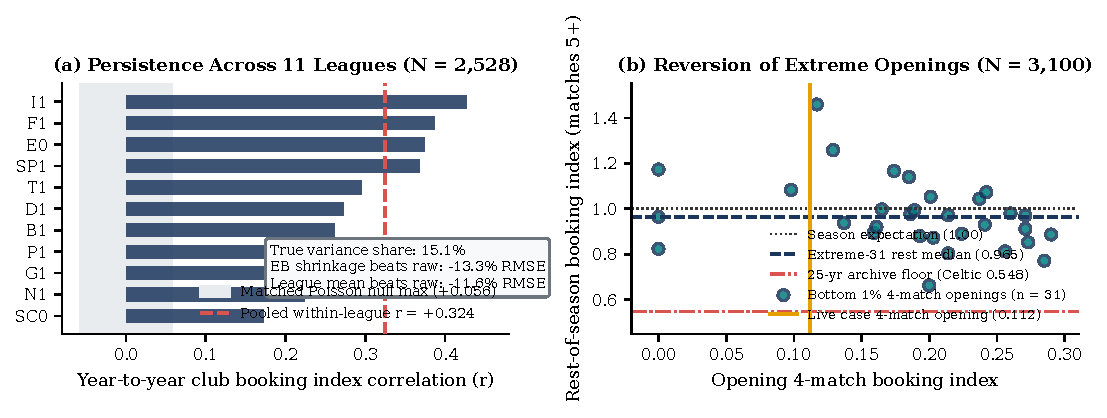
\includegraphics[width=\textwidth]{figures/fig4.pdf}
\caption{\textbf{Study 04 \& Sealed Out-of-Sample Protocol: Persistence, Empirical-Bayes shrinkage, and reversion of extreme openings.} \textbf{(a)} Year-to-year club booking index persistence across $2,528$ consecutive club-season pairs in $11$ leagues ($r = +0.324, p = 6.5\times 10^{-63}$, positive in $11/11$ leagues vs.\ $2,000$-draw matched Poisson null maximum $+0.056$); only $15.1\%$ of single-season variance is true club signal ($\sigma_{\text{true}} = 0.051$). \textbf{(b)} Across $3,100$ completed team-seasons, all $31$ bottom-$1\%$ four-match openings (index $\le 0.292$) reverted over the remainder of the season to a median index of $0.965$ and a minimum of $0.663$ (above the $25$-year archive floor of $0.548$).}
\label{fig:fig4}
\end{figure*}

To determine how much of a single season's adjusted booking index reflects a repeatable club trait versus Poisson sampling noise, we constructed $2,528$ consecutive same-division club-season pairs ($\ge 25$ matches per season) across all $11$ leagues in our $58,013$-match archive.

\subsection{Persistence, Poisson Null, and Variance Decomposition}
Across the $2,528$ consecutive pairs, a club's situation- and era-adjusted booking index in season $t$ correlates with its index in season $t+1$ at $r = \mathbf{+0.324}$ ($R^2 = 10.5\%, p = 6.5\times 10^{-63}$), and is positive in $\mathbf{11}$ of $\mathbf{11}$ leagues (ranging from $+0.172$ in Scotland to $+0.427$ in Italy; Figure~\ref{fig:fig4}(a)). Resampling each club-season's yellow cards $2,000$ times from $\text{Poisson}(\text{expected}_{i,s})$ while holding fixture lists and expectations fixed produces a matched null with $\bar{r} = -0.0004$, $95\text{th}$ percentile $+0.032$, and a maximum across all $2,000$ draws of $\mathbf{+0.056}$ ($p < 0.0005$).

Decomposing the observed cross-sectional variance $\sigma^2_{\text{obs}} = 0.01735$ into expected Poisson sampling variance $\sigma^2_{\text{Poisson}} = E[Y / E[Y]^2] = 0.01473$ and true club heterogeneity $\sigma^2_{\text{true}} = \sigma^2_{\text{obs}} - \sigma^2_{\text{Poisson}} = 0.00262$ reveals that only $\mathbf{15.1\%}$ of the spread in single-season booking indices is a true club property ($\sigma_{\text{true}} = \mathbf{0.051}$), while $\mathbf{84.9\%}$ is the random Poisson noise of one season's cards.

\subsection{Out-of-Sample Shrinkage Validation}
Because single-season reliability is $0.151$, ranking clubs on one season of unshrunk ratios is dominated by estimation error. Across $2,432$ consecutive club-season pairs ($\ge 30$ matches), we evaluated three forecasts of a club's season-$t+1$ booking rate: (i) the club's own season-$t$ raw ratio, (ii) the league mean (ignoring the club entirely), and (iii) an Empirical-Bayes Beta-Binomial shrunken estimator $\hat{\theta}_i = \frac{n_i}{n_i + n_0} r_i + \frac{n_0}{n_i + n_0} \bar{r}_L$ \citep{efron1975stein,brown2008season}. Out-of-sample RMSE is $0.0267$ for the club's raw ratio, $0.0236$ for the league mean, and $0.0232$ for the shrunken estimate: \textbf{ignoring the club and predicting the league mean beats the club's own one-season ratio by $11.6\%$}, and \textbf{Empirical-Bayes shrinkage beats the raw ratio by $13.3\%$}.

\subsection{Sealed Four-Match Protocol and Historical Reversion}
At the start of the $2026\text{--}27$ Portuguese season (snapshot \texttt{2026-W36}, $33$ matches through matchweek $4$), FC Porto committed $58$ fouls and received $1$ yellow card across $4$ matches. Under our frozen pre-registered affine model ($1.1259 + 0.095491 \times \text{fouls}$) and heavy-favourite multiplier ($0.830$), expected cards fell from $10.04$ (era-only) to $8.34$, yielding an adjusted index of $\mathbf{0.120}$ ($95\%$ CI $[0.003, 0.668]$), the sole club among $18$ surviving a Benjamini--Hochberg screen at $\text{FDR} = 0.10$ ($p_{\text{BH}} = 0.081$ vs.\ $0.017$ without the favourite adjustment). Applying the most generous spatial placement ceiling observed across the five European event-data leagues (Spain's $7.3\%$ reduction) moves expected cards only from $8.34$ to $7.73$ (index $0.129, p = 0.0077$), accounting for just $\mathbf{1.1\%}$ of the $88.0\%$ shortfall.

To establish the historical base rate without waiting for season completion, we severed all $3,100$ completed team-seasons in our $11$-league archive after match $4$ (Figure~\ref{fig:fig4}(b)). Across all $3,100$ team-seasons, the four-match opening index correlates with the rest-of-season index (matches $5+$) at only $r = \mathbf{+0.118}$. Exactly $4$ historical openings were at least as extreme as Porto's unadjusted opening ($0.112$), and the most lenient $1\%$ ($\le 0.292$, $31$ team-seasons) finished with a rest-of-season median index of $\mathbf{0.965}$ and a minimum of $\mathbf{0.663}$---none approaching the $25$-year full-season archive floor (Celtic $2024\text{--}25$ at $0.548$). On 30 August 2026, we sealed a prospective decision rule on Porto's yellow-card total over the subsequent seven matchweeks (matchweeks $4\text{--}10$, resolving 15 November 2026): $\le 7$ yellows classifies the run as persistent ($22.6\%$ historical base rate among the $31$ extreme openings vs.\ $0.62\%$ in Portugal, where the median seven-match stretch is $19$ cards and Porto's nine-season historical minimum is $14$), $8\text{--}11$ as ambiguous ($29.0\%$), and $\ge 12$ as noise ($48.4\%$).

\section{Conclusion}

Across $58,013$ matches and $47,955$ spatio-temporally coded fouls, apparent club-level disciplinary anomalies dissolve when subjected to proper statistical controls. Raw cards-per-foul ratios confound club identity with match-winner expectation ($31.3\%$ swing), non-foul conduct intercepts ($13\%\text{--}47\%$ of bookings), and fixture-level intensity shared with the opponent ($r = +0.283$). At the event level, the $3.5$-fold spatial card gradient goes largely unexploited across clubs because team foul distributions compress into a narrow midfield band ($[48.2, 58.0]$), and at the season level, $84.9\%$ of cross-sectional variance is Poisson noise, making Empirical-Bayes shrinkage mandatory before any disciplinary ranking is interpreted.

{\small
\bibliographystyle{plainnat}
\bibliography{references}
}

\end{document}
